\documentclass[tikz, border=5pt]{standalone}
\usepackage{tikz}
\usetikzlibrary{arrows.meta, positioning}

\definecolor{myred}{RGB}{200, 50, 50}
\definecolor{myblue}{RGB}{50, 100, 200}

\begin{document}

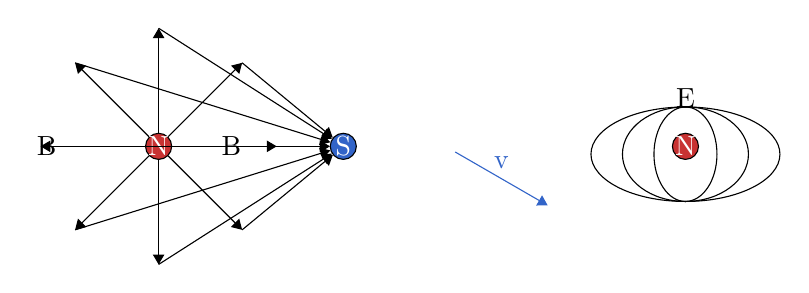
\begin{tikzpicture}[node distance=2cm]

    % North Pole Diagram
    \node[draw, circle, fill=myred] (N) {};
    \node at (N) [text=white] {N};

    \foreach \angle in {0, 45, ..., 315}
    {
        \draw[-{Triangle}] (N) -- ++(\angle:1.5cm);
    }

    \node[left=1cm of N] (B1) {B};

    % South Pole Diagram
    \node[draw, circle, fill=myblue, right=of N] (S) {};
    \node at (S) [text=white] {S};

    \foreach \angle in {0, 45, ..., 315}
    {
        \draw[-{Triangle}] ++(\angle:1.5cm) -- (S);
    }

    \node[left=1cm of S] (B2) {B};

    % Electric field
    \node[draw, circle, fill=myred, right=4cm of S] (EN) {};
    \node at (EN) [text=white] {N};

    \node[above=0.2cm of EN] (E) {E};

    \foreach \radius in {0.4, 0.8, 1.2}
    {
        \draw[-{Triangle}] ([yshift=-0.1cm]EN) +(0,0) ellipse (\radius cm and 0.6cm);
    }

    % Velocity
    \node[right=1cm of S] (V) {};
    \draw[-{Triangle}, myblue] (V) -- ++(-30:1.5cm) node[midway, above] {v};

\end{tikzpicture}

\end{document}
